%-------------------------------------------------------------------------------
%-------------------------------------------------------------------------------
\section{Intégrales}
%-------------------------------------------------------------------------------

% Jacobien et changement de variables en dimension supérieure ou égale à 2.

% \begin{theorem*}{Fubini-Tonelli}
% \end{theorem*}
% 
% \begin{theorem*}{Fubini-Lebesque}
% \end{theorem*}

%-------------------------------------------------------------------------------
\subsection{Difféomorphisme}
%-------------------------------------------------------------------------------

\begin{definition*}[Difféomorphisme]
  Soient $\Xcal$ et $\Ycal$ deux ouverts de $\Rbb^n$ et une bijection $g : \Xcal \mapsto \Ycal$. $g$ est un difféomorphisme si $g$ est différentiable partout dans $\Xcal$ et que $g^{-1}$ est différentiable partout dans $\Ycal$. \\
  Si, de plus, les dérivées partielles de $g$ et $g^{-1}$ sont partout continues, $g$ est un $C^1$-difféomorphisme.
\end{definition*}

%-------------------------------------------------------------------------------
\paragraph{Différentielle de la réciproque.}
Si $g : \Xcal \mapsto \Ycal$ est un difféomorphisme, puisque $g^{-1} \circ g = Id$ et que $D_x Id = I_n$, on a
$$
I_n = D_x(g^{-1} \circ g) = D_{g(x)}(g^{-1}) D_x g 
\qquad \text{(par composition)},
$$
soit
$$
D_{g(x)}g^{-1} = (D_x g)^{-1}.
$$
On retrouve ainsi la formule valable dans $\Rbb$ :
$$
(g^{-1})'(y) = 1 /g'(x)
\qquad \text{ou} \quad x = g^{-1}(y).
$$

\begin{theorem*}[Inversion globale]
  Soit $\Xcal$ un ouvert de $\Rbb^n$ et $g : \Xcal \mapsto \Rbb$. Supposons que $g$ est injective, différentiable sur tout $\Xcal$ et que ses dérivées partielles sont partout continues dans $\Xcal$. Si, de plus, $D_x g$ est inversible sur tout $\Xcal$, alors $g : \Xcal \mapsto \Ycal = g(\Xcal)$ est un $C^1$-difféomorphisme.
\end{theorem*}

\proof Non démontré. \eproof

\remark
Ce théorème assure le $C^1$-difféomorphisme sans exiger la différentiabilité continue de $g^{-1}$.

%-------------------------------------------------------------------------------
\subsection{Jacobien, changement de variable}
%-------------------------------------------------------------------------------

\begin{definition*}[Jacobien]
  Pour $g : \Rbb^n \mapsto \Rbb^n$, le jacobien de $f$ au point $x$ est le déterminant de sa matrice jacobienne au point $x$ : 
  $$
  \det(J_x f).
  $$
\end{definition*}

\remark
Le jacobien d'un difféomorphisme ne peut pas être nul, puisqu'un difféomorphisme est bijectif.

\begin{theorem*}[Changement de variable]
  Soit $\Xcal$ et $\Ycal$ deux ouverts de $\Rbb^n$ et $g : \Xcal \mapsto \Ycal = g(\Xcal)$ un $C^1$-difféomorphisme et $f : \Ycal \mapsto \Rbb^+$, on a 
  $$
  \int_\Ycal f(y) \; \d y = \int_\Xcal f \circ g(x) |\det(J_x g)| \; \d x.
  $$
\end{theorem*}

\proof
Non démontrée : la preuve passe par le découpage du domaine d'intégration en fonction des différents type d'action de la matrice jacobienne $J_x g$ (transvection, permutation ou
dilatation).
\eproof

\remark
La contrainte de signe pour $f$ assure que le résultat de l'intégration ne dépend pas de l'ordre selon lequel on intègre par rapport aux différente coordonnée (théorème Fubini-Tonelli). Le théorème de Fubini-Lebesgue lève cette contrainte mais requiert que $f$ soit bornée.

\begin{corollary*}[Coordonnées polaires]
  Pour tout $f : \Rbb^2 \mapsto \Rbb^+$, 
  $$
  \int_\Rbb \int_\Rbb f(x, y) \; \d x \d y
  = \int_{\Rbb^+} \int_0^{2 \pi} f(\rho \cos \theta, \rho \sin \theta) \rho \; \d \rho \d \theta
  $$
\end{corollary*}

\proof
\begin{itemize}
  \item On a vu que $f$ est partout différentiable et que $|J_{(\rho, \theta)}f| = \rho$.
  \item On vérifie facilement que $g$ est bijective et que ses dérivées partielles sont partout continues.
\end{itemize}
\eproof

\begin{exercise*}
  On veut calculer 
  $$
  I = \int_\Rbb e^{-x^2} \; \d x.
  $$
  \begin{itemize}
    \item En utilisant un passage en coordonnées polaires, calculer
    $$
    J = \int_\Rbb \int_\Rbb e^{-(x^2+y^2)} \; \d x \; \d y.
    $$
    \item Montrer que, de plus, $J = I^2$ et conclure.
  \end{itemize}
\end{exercise*}

%-------------------------------------------------------------------------------
%-------------------------------------------------------------------------------
\section{Extremums}
%-------------------------------------------------------------------------------

%-------------------------------------------------------------------------------
\subsection{\textcolor{gray}{Variétés}}
%-------------------------------------------------------------------------------

\textcolor{gray}{Courbe de niveau (cf notes manuscrites, dans section chgt de variable)}

%-------------------------------------------------------------------------------
\subsection{Extrema}
%-------------------------------------------------------------------------------

\begin{definition*}[Gradient]
  Soit $f : \Rbb^k \mapsto \Rbb$ différentiable en $x^*$, le gradient de $f$ en $x^*$ est le vecteur constitué de ses dérivées partielles évaluées en $x^*$ : 
  $$
  \nabla_{x^*}f 
  = \left[\begin{array}{c}
              \displaystyle{\left.\frac{\partial f}{\partial x_1}\right|_{x^*}}  \\
              \vdots \\
              \displaystyle{\left.\frac{\partial f}{\partial x_k}\right|_{x^*}} 
             \end{array}\right]
  = \left[J_{x^*} f\right]^\top.
  $$
\end{definition*}

\remark
\begin{enumerate}
  \item Si $f$ est différentiable en $x$, on a
  $$
  f(x + h) = f(x) + \nabla_{x^*}f^\top h + o(\|h\|).
  $$
  \item Un point $x$ pour lequel le gradient de $f$ est nul est appelé {\em point stationnaire} (ou {\em point critique}) de $f$ : au premier ordre, la fonction $f$ est constante au voisinage de $x$.
\end{enumerate}


\begin{definition*}[Matrice hessienne]
  Soit $f : \Rbb^k \mapsto \Rbb$ différentiable en $x^*$, la matrice hessienne ('la hessienne') $f$ en $x^*$ est la matrice ayant pour éléments génériques les dérivées secondes croisées évaluées en $x^*$ : 
  $$
  \nabla^2_{x^*}f 
  = \left[\left.\frac{\partial^2 f}{\partial x_i\partial x_j}\right|_{x^*} \right]_{1 \leq i, j \leq k}
%   = \left[\begin{array}{ccc}
%               \displaystyle{\left.\frac{\partial^2 f}{\partial x_1^2}\right|_{x^*}} & 
%               \cdots & 
%               \displaystyle{\left.\frac{\partial^2 f}{\partial x_1\partial x_k}\right|_{x^*}} \\
%               \vdots & 
%               \displaystyle{\left.\frac{\partial^2 f}{\partial x_i\partial x_j}\right|_{x^*}}\vdots & 
%               \\
%               \displaystyle{\left.\frac{\partial^2 f}{\partial x_k\partial x_1}\right|_{x^*}} & 
%               \cdots & 
%               \displaystyle{\left.\frac{\partial^2 f}{\partial x_k^2}\right|_{x^*}}
%           \end{array} \right].
  $$
  Les termes diagonaux de $\nabla^2_{x^*}f$ sont les dérivées secondes par rapport à chacune des coordonnées : 
  $$
  \left[ \nabla^2_{x^*}f \right]_{ii} 
  = \left.\frac{\partial^2 f}{\partial x_i^2}\right|_{x^*}.
  $$
  $\nabla^2_{x^*}f$ est notamment symétrique, ce qui implique qu'elle est diagonalisable.
\end{definition*}

\begin{proposition*}
  Si $f$ est deux fois différentiable en $x$, alors
  $$
  f(x+h) = f(x) + \nabla_x f^\top \cdot h + \frac12 h^\top \cdot \nabla^2_x f \cdot h + o(\|h\|^2).
  $$
\end{proposition*}

\proof Non démontrée. \eproof

\remark
\begin{itemize}
 \item $f$ est deux fois différentiable en $x$ signifie que $f$ est différentiable en $x$ et que l'application $g$ de $\Rbb^k$ dans $\Rbb^k$ définie par $g(x) = \nabla_x f$ est elle-même différentiable en $x$.
 \item Ce résultat étend la formule de Taylor à l'ordre 2 pour une fonction $f : \Rbb \mapsto \Rbb$ : 
 $$
 g(u+t) = g(u) + g'(y) t + \frac12 g''(u) t^2 + o(t^2).
 $$
 Une preuve de la proposition précédente peut être établie en appliquant la formule de Taylor pour une fonction de $\Rbb$ dans $\Rbb$ à la fonction $g_{x, h}(t) = f(x + th)$.
\end{itemize}


\begin{definition*}[Extremum local]
  Si $f$ est deux fois différentiable en $x$ et que son gradient y est nul : $\nabla_xf = 0$, alors
  \begin{itemize}
   \item $x$ est {\em maximum local} si $\nabla^2_x f$ est définie négative et
   \item $x$ est {\em minimum local} si $\nabla^2_x f$ est définie positive.
  \end{itemize}
  Dans les deux cas, $x$ est un {\em optimum relatif}.
\end{definition*}

\remark
Puisque le gradient $\nabla_x f$ est nul, on a au voisinage de $x$ :
$$
f(x+h) - f(x) \simeq \frac12 h^\top \cdot \nabla^2_x f \cdot h.
$$
Un maximum (resp. minimum) se caractérise par le fait que la fonction $f$ diminue (resp. augmente) dans toutes les directions $h$. Le fait que $\nabla^2_x f$ soit définie négative (resp. positive) assure précisément que $f(x+h) - f(x)$ est négatif (resp. positif) dans tout le voisinage de $x$.

%-------------------------------------------------------------------------------
\subsection*{Cas de $f : \Rbb^2 \mapsto \Rbb$}
%-------------------------------------------------------------------------------

\begin{definition*}[Notation de Monge]
  Pour $f : \Rbb^2 \mapsto \Rbb$, on note les dérivées au point $a = (x^*, y^*) \in \Rbb^2$
  \begin{align*}
    p & = \left.\frac{\partial f}{\partial x}\right|_a, &
    q & = \left.\frac{\partial f}{\partial y}\right|_a, &
    r & = \left.\frac{\partial^2 f}{\partial x^2}\right|_a, &
    s & = \left.\frac{\partial^2 f}{\partial x \partial y}\right|_a, &
    t & = \left.\frac{\partial^2 f}{\partial y^2}\right|_a
  \end{align*}
  c'est à dire
  $$
  \nabla_af = \left[\begin{array}{c} p \\ q \end{array} \right], 
  \qquad 
  \nabla^2_af = \left[\begin{array}{cc} r & s \\ s & t \end{array} \right].
  $$
\end{definition*}

%-------------------------------------------------------------------------------
\paragraph{Caractérisation des optimums.}
Toutes les valeurs propres d'une matrice définie positive ou négative sont de même signe. 
En dimension deux, cela signifie que leur produit est positif.
$a = (x^*, y^*)$ est donc un optimum relatif de $f$ si le déterminant de la hessienne de $f$ en $a$ est positif : 
$$
|\nabla^2_a f| = rt - s^2 > 0
\qquad \Rightarrow \qquad
\text{$a$ est un optimum local} .
$$
Le cas $|\nabla^2_a f| = rt - s^2 > 0$ correspond au cas où les deux valeurs propres sont de signe opposé, c'est-à-dire que $a$ est un maximum dans une direction et un minimum dans une autre : on parle alors de point selle.

\progres{
  Début Cours 7. Rappels :
  \begin{enumerate}[\itemdot]
    \item Changement de variables
    $$
    \int_{\Rbb^n} f(y) \; \d y = \int_{\Rbb^n} f \circ g (x) \; |J_x g| \; \d x
    $$
    $|J_x g| =$ jacobien de $g$ au point $x$.
    \item Extrema
    $$
    f(x+h) = f(x) + (\nabla_x f)^\top h + \frac12 h^\top (\nabla^2_x f) h + o(\|h\|^2).
    $$
    $x =$ extremum local si $\nabla_x f = 0$, maximum si $\nabla^2_x f \preccurlyeq 0$, minimum si $\nabla^2_x f \succcurlyeq 0$.
    \item Cas particulier $\Rbb^n = \Rbb^2$ : caractérisation des extrémum à partir du déterminant et de la trace de $\nabla^2_x f$.
    \item Exercice maison.
  \end{enumerate}
}

\begin{exercise*}[A faire à la maison]
  Déterminer les points stationnaires de la fonction 
  $$
  f(x, y) = x^3 + y^3 - 3 xy
  $$
  déterminer s'il s'agit de maximums, de minimums ou de points selles.
\end{exercise*}

\solution{
  \begin{description}
    \item[Points critiques :] Le gradient de $f$ vaut
    $$
    \nabla f = \left[\begin{array}{c} 3x^2 - 3y \\ 3y^2 - 3x \end{array}\right]
    $$
    qui est nul aux points
    $$
    a = (0, 0) \qquad \text{et} \qquad b = (1, 1).
    $$
    De plus la hessienne vaut
    $$
    \nabla^2 f = \left[\begin{array}{rrr} 6x & & -3 \\ -3 & & 6y \end{array}\right].
    $$
    %
    \item[\'Etude du point $a$ :] on a 
    $$
    \nabla_a^2 f = \left[\begin{array}{rrr} 0 & & -3 \\ -3 & & 0 \end{array}\right]
    \qquad \Rightarrow \qquad 
    | \nabla_a^2 f | = -9 < 0
    $$
    donc $a$ est un point selle. Ses valeurs propres sont les racines de
    $$
    P(\lambda) = \left|\begin{array}{rrr} -\lambda & & -3 \\ -3 & & -\lambda \end{array}\right|
    = \lambda^2 - 9 
    \qquad \text{soit} \quad 
    \lambda = \pm 3.
    $$
    Tout vecteur propre associé à $\lambda = -3$ est solution de 
    $$
    \left\{\begin{array}{rcl} -3y & = & -3x \\-3x & = & -3y\end{array} \right.
    \qquad \Rightarrow \qquad 
    x = y
    \qquad \Rightarrow \qquad 
    \left[ \begin{array}{r} 1 \\ 1 \end{array} \right] \text{ est associé à $-3$}
    $$
    donc $a$ est un maximum dans la direction de la 1ère bissectrice. \\
    Tout vecteur propre associé à $\lambda = 3$ est solution de 
    $$
    \left\{\begin{array}{rcl} -3y & = & 3x \\-3x & = & 3y\end{array} \right.
    \qquad \Rightarrow \qquad 
    x = -y
    \qquad \Rightarrow \qquad 
    \left[ \begin{array}{r} -1 \\ 1 \end{array} \right] \text{ est associé à $+3$}
    $$
    donc $a$ est un minimum dans la direction de la 2ème bissectrice.
    %
    \item[\'Etude du point $b$ :] on a
    $$
    \nabla_b^2 f = \left[\begin{array}{rrr} 6 & & -3 \\ -3 & & 6 \end{array}\right]
    \qquad \Rightarrow \qquad 
    | \nabla_b^2 f | = 27 > 0
    $$
    donc $b$ est un optimum. Comme de plus la trace de $\nabla_b^2 f$ vaut 12, ses deux valeurs propres sont positives : $b$ est donc un minimum.
  \end{description}
}

\dessin{
\paragraph{Fonction $f(x, y) = x^3 + y^3 - 3xy$:}
$$
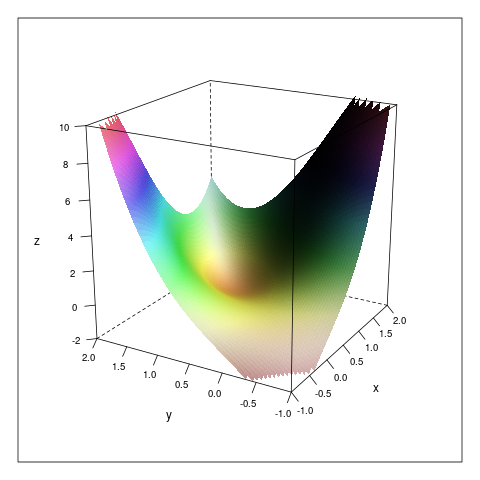
\includegraphics[width=.6\textwidth]{ExempleOptimum-surface}
$$
\paragraph{Point $a = (0, 0)$:}
$$
\begin{tabular}{cc}
  direction $x = y$ & direction $x = -y$ \\
  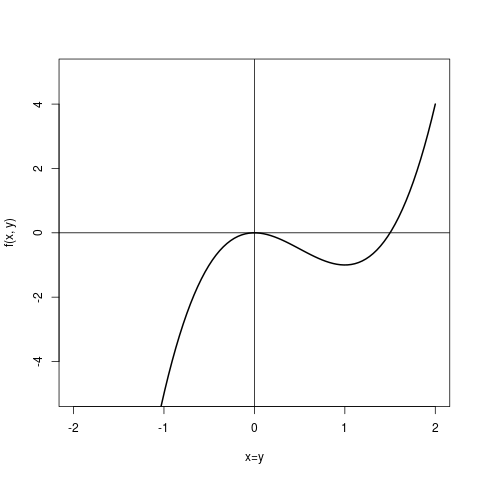
\includegraphics[width=.4\textwidth]{ExempleOptimum-1ereBissectrice} &
  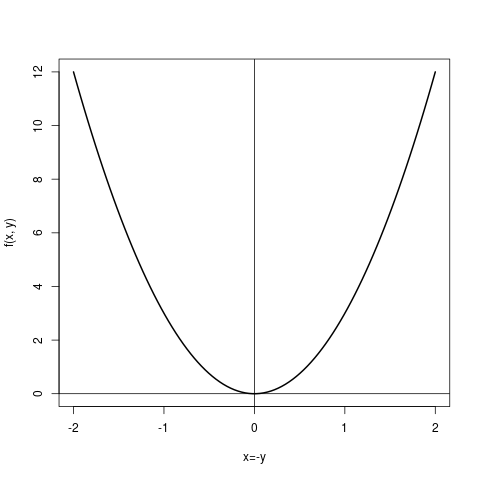
\includegraphics[width=.4\textwidth]{ExempleOptimum-2emeBissectrice} \\
  $f(x, x) = 2x^3 - 3x^2$ & $f(x, -x) = 3x^2$
\end{tabular}
$$
}
